\begin{figure*}[!t]
    \centering
    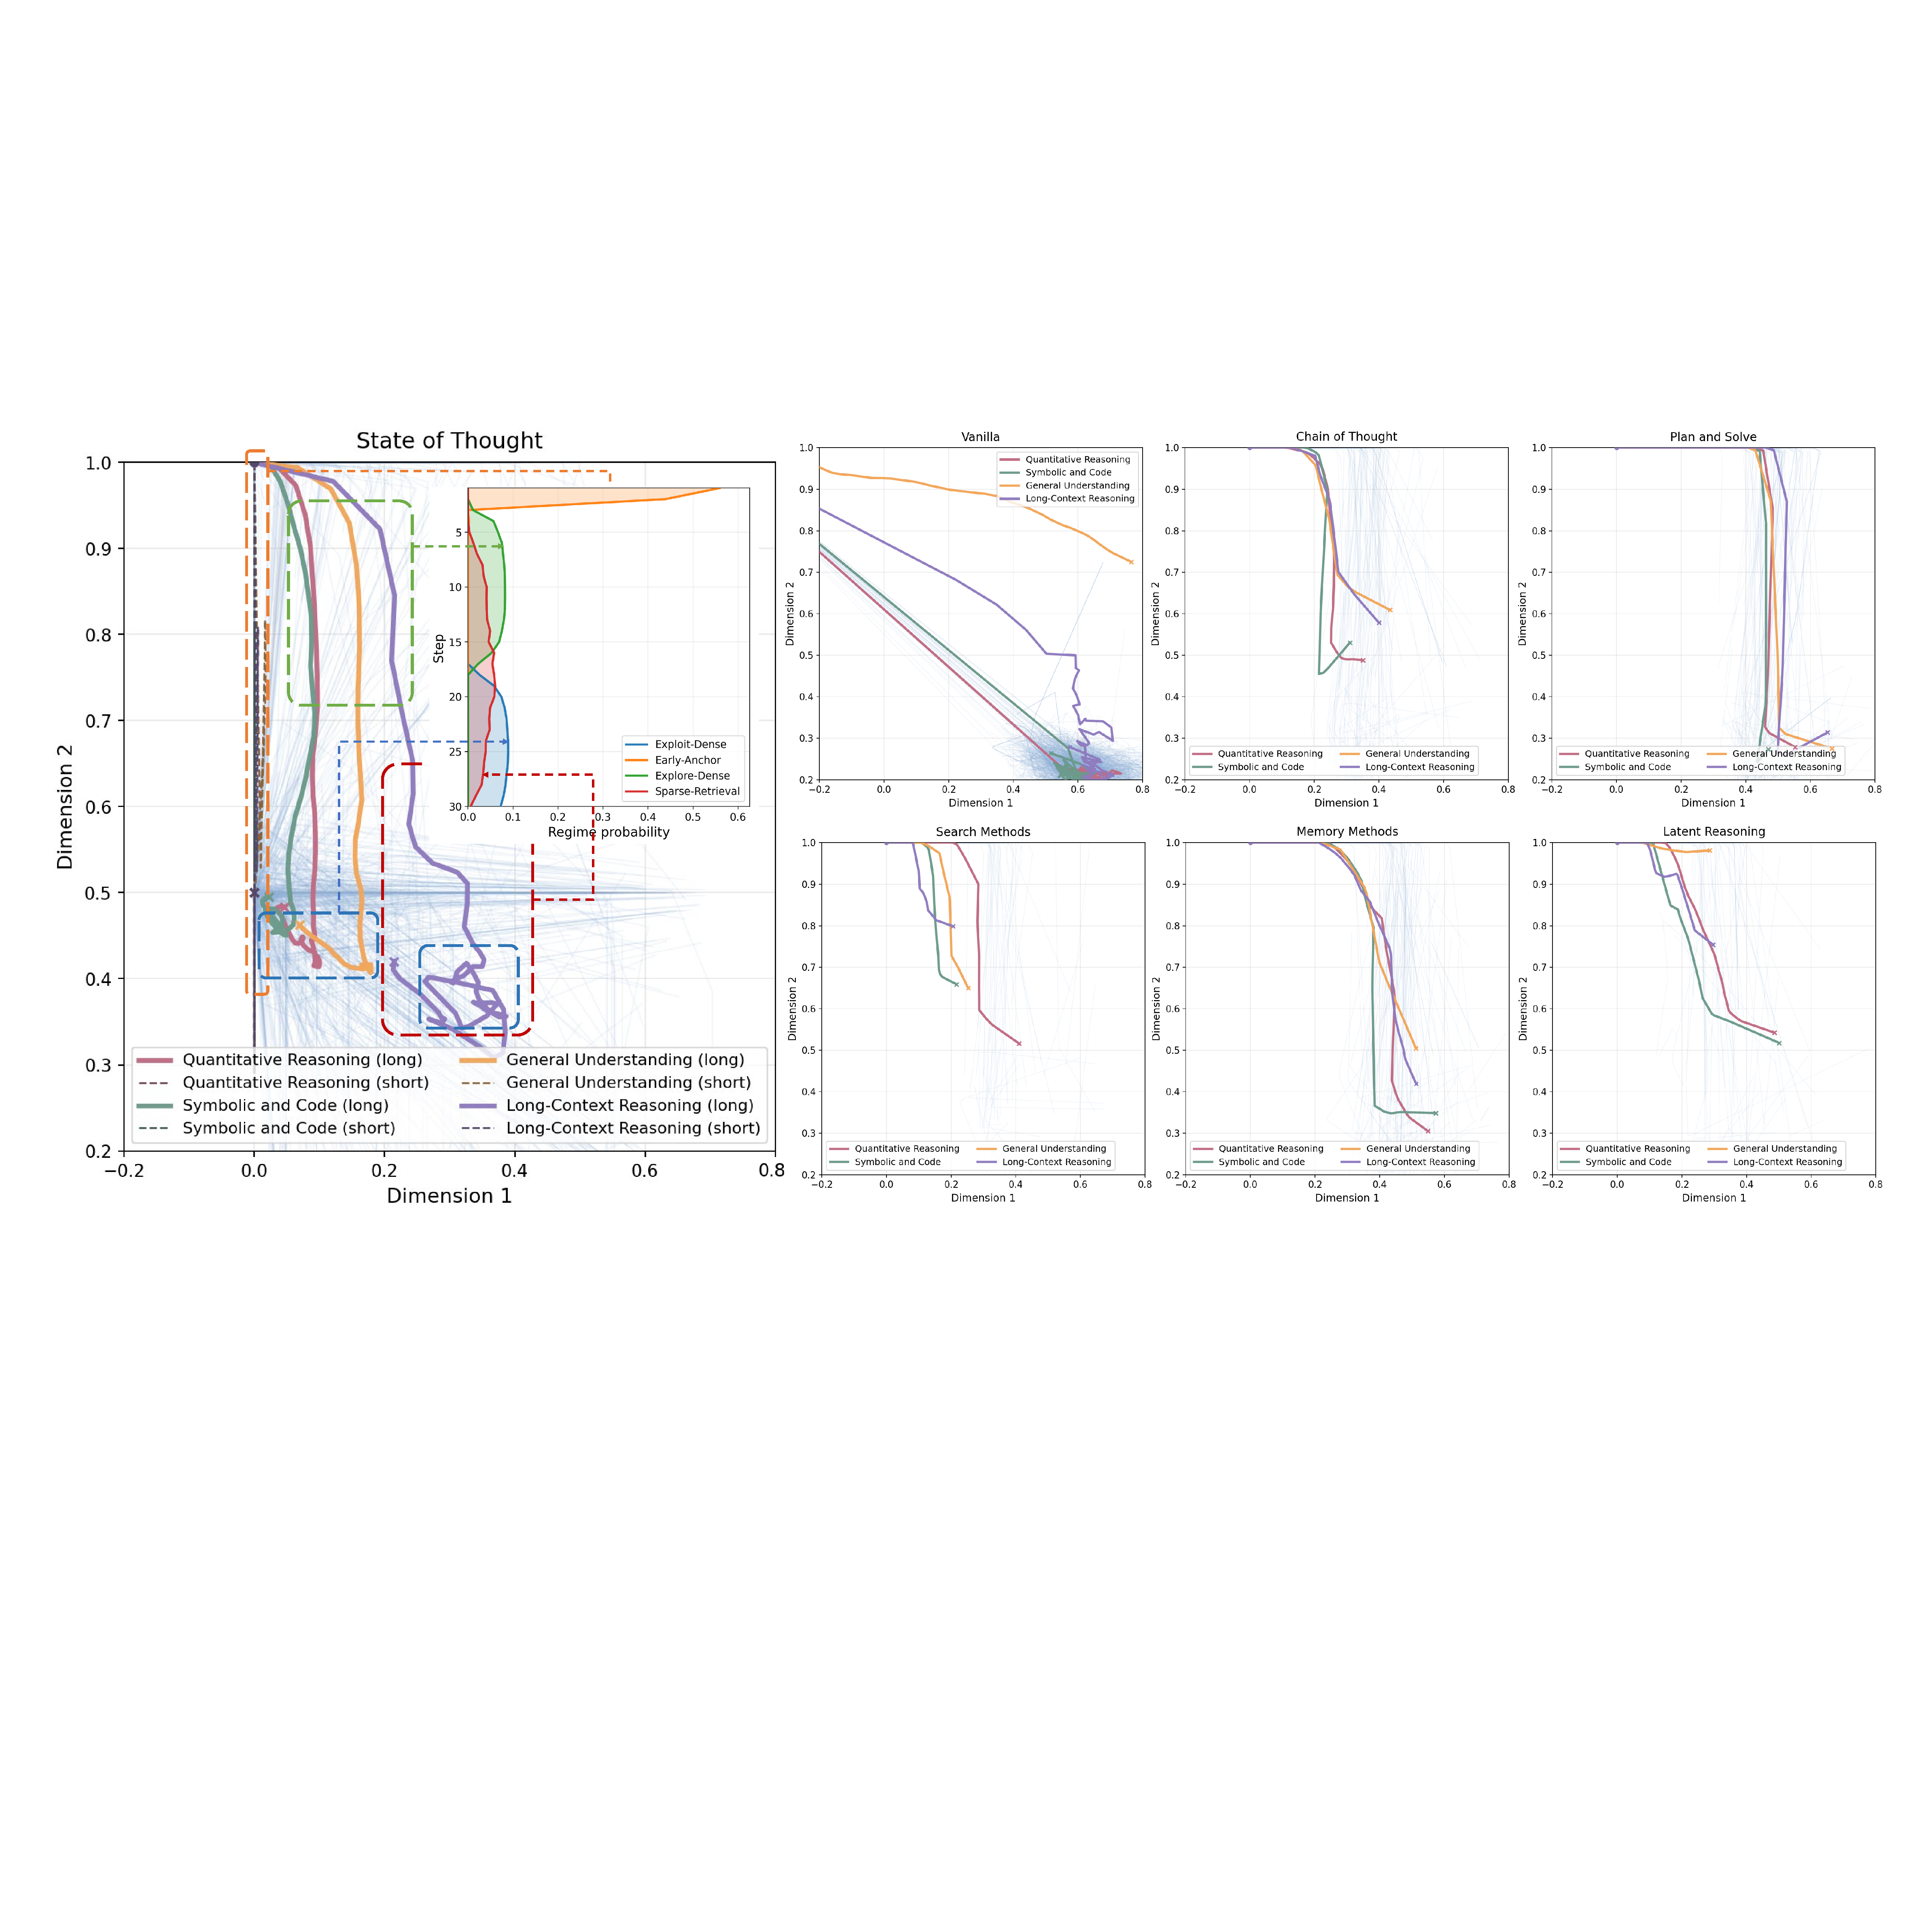
\includegraphics[width=1.0\textwidth]{figs/state_space_regimes.pdf}
    \caption{
    \textbf{Endogenous reasoning state trajectories across various reasoning paradigms} on Llama-3.1-8B with breakdown in Figure~\ref{fig:app_state_regimes} and reasoning state definition in Figure~\ref{fig:state_conditioned_activation}.
    Different externally induced reasoning strategies occupy distinguishable regions in the dynamics-geometric state space, while SoT supports a broader and more adaptive state distribution.
    }
    \vspace{-3mm}
    \label{fig:state_space_regimes}
\end{figure*}

\section{State of Thought}
\label{sec:method}

\subsection{Problem Formulation}
\label{sec:problem_formulation}

We formulate test-time reasoning of a frozen autoregressive LLM \(f\) as a policy-governed multi-step trajectory generation started from a problem \(x\) presented by prompt \(p\) \citep{brown2024large}.
The model \(f\) dynamically generates the subsequent reasoning trajectory \(y_{1:T}=(y_1,\dots,y_T)\) leading to the final answer \(a\):
\begin{equation}
\mathbb{P}_{\pi}(a, y_{1:T}\mid p)
=
\prod_{t=1}^{T} \mathbb{P}_{\pi}(y_t \mid p,y_{<t})\;
\mathbb{P}_{\pi}(a \mid p,y_{1:T}),
\end{equation}
with the policy \(\pi\) determining how evidence from prior steps is organized for subsequent decisions, while different reasoning paradigms differ in prompt construction and policy \citep{snell2024scaling}.

State of Thought seeks such a policy that the model's current endogenous state (Sec.~\ref{sec:endogenous_state}) governs both evidence-context organization and reasoning continuation (Sec.~\ref{sec:state_driven_activation}), with no external reasoning instructions imposed on the prompt.

\subsection{Endogenous Reasoning State}
\label{sec:endogenous_state}

Effective reasoning policy \(\pi\) should be governed not by external scripts but by a compact endogenous state that reflects the geometry and dynamics of ongoing reasoning \citep{park2025geometry,park2024linear,zou2023repe}. Accordingly, we read out a compact \emph{dynamics-geometric state} \(m_t \in \mathbb{R}^4\) from the model's internal information transfer of sentence-level reasoning unit \(y_t\) with calculation details in Appendix~\ref{app:endogenous_state}:
\begin{equation}
m_t = \big[\delta_t,\; v_t,\; c_t,\; H_t\big],
\label{eq:sot_state}
\end{equation}
where \(\delta_t\) characterizes the internal organization distinguishing concentrated from diffuse local structure; \(v_t\) captures stepwise progress through magnitude; \(c_t\) captures directional consistency distinguishing stable continuation from deviation or redirection; and \(H_t\) measures the model's local predictive uncertainty. Together, these four quantities summarize the current reasoning endogenous control state and condition how the evidence context should be organized for subsequent decisions.

\paragraph{Interpretability of endogenous reasoning state.}
To verify that \(m_t\) can capture reasoning-relevant internal structure rather than arbitrary hidden variation, we aggregate trajectories from multiple external reasoning paradigms in the constructed state space in Figure~\ref{fig:state_space_regimes}. 
SoT spans a broader and more adaptive state distribution, while others with externally structured reasoning programs occupy distinguishable regions, collapsing to fixed scripted patterns. 
This indicates that SoT is less constrained by externally imposed reasoning formats and more aligned with the model's endogenous state evolution, enabling stronger generalization across heterogeneous reasoning structures.

\begin{figure*}[!t]
    \centering
    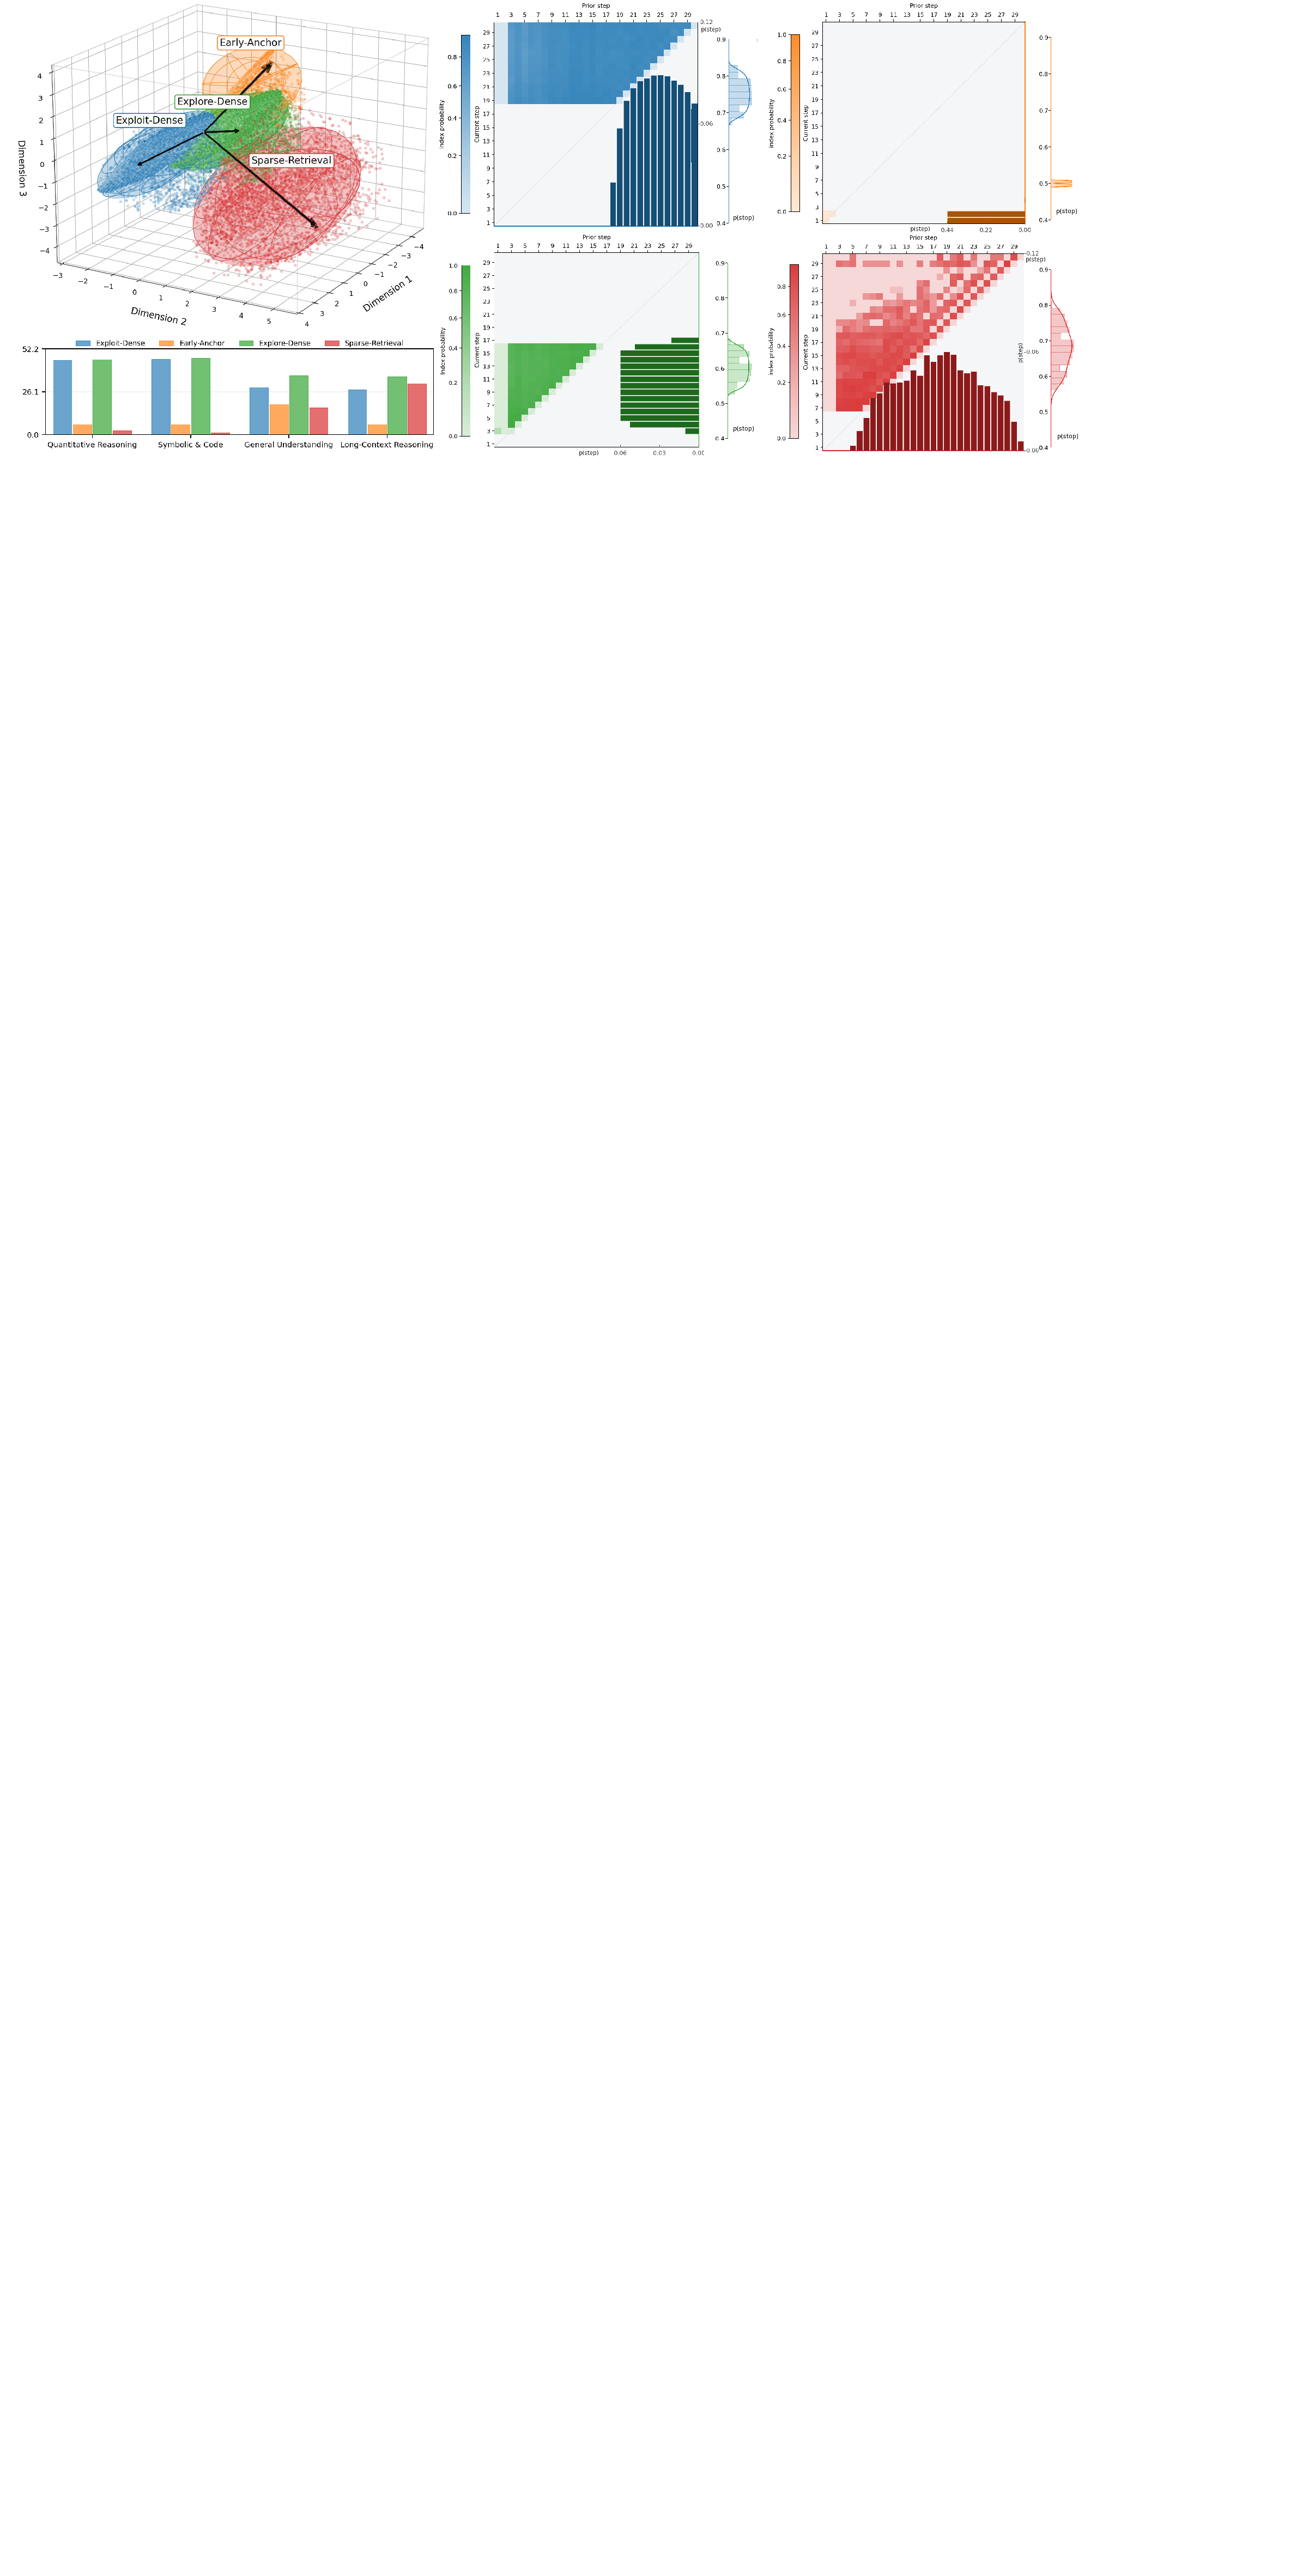
\includegraphics[width=1.0\textwidth]{figs/state_conditioned_activation.pdf}
    \caption{
    \textbf{State-conditioned reasoning in SoT} with breakdown in Figure~\ref{fig:app_state_clusters}.
    Different endogenous reasoning states induce different sparse activation patterns and different stop tendencies.
    }
    \vspace{-3mm}
    \label{fig:state_conditioned_activation}
\end{figure*}

\subsection{State-Conditioned Reasoning}
\label{sec:state_driven_activation}

SoT instantiates the reasoning policy \(\pi\) through evidence-organization operator \(\mathcal{S}\) and stopping operator \(\mathcal{T}\) as two state-conditioned operators with details in Appendix~\ref{app:sot-details}.

\emph{State-conditioned evidence selection.}
Given the current state \(m_t\) and the historical reasoning trajectory \(y_{<t}\), the evidence-organization operator \(\mathcal{S}\) selects the reasoning-related sparse subset \(\widetilde{y}_{<t}=\mathcal{S}(y_{<t};m_t)\subset y_{<t}\) as the evidence context for subsequent reasoning to generate the next step
\begin{equation}
\mathbb{P}_{\pi}(y_t \mid p,y_{<t}) = \mathbb{P}\!\left(y_t \mid p,\widetilde{y}_{<t}\right),
\label{eq:state_policy_select}
\end{equation}
% so that subsequent reasoning depends not on the full history \citep{li2023compressing} or a generic relevance heuristic \citep{packer2023memgpt}, but on the evidence context selected under the current endogenous state. 
In this way, SoT improves reasoning not by broadening search over more trajectories \citep{yao2023tree}, but by sharpening the evidence context carried into the next decision.

\emph{State-conditioned stopping.}
SoT also produces a continuation decision \(z_t=\mathcal{T}(m_t)\in\{0,1\}\), where \(z_t=0\) continues reasoning and \(z_t=1\) terminates reasoning and triggers final answer generation as
\begin{equation}
\mathbb{P}_{\pi}(a \mid p,y_{1:t}) = \mathbb{P}(a \mid p,\widetilde{y}_{<t}, y_t).
\label{eq:state_policy_step}
\end{equation}
Stopping therefore emerges from the current reasoning endogenous state rather than from a fixed external schedule \citep{hosseini2026early} on reasoning depth.

Overall, SoT treats evidence sparsification and stopping as two outputs of the same endogenous reasoning policy: one determines what evidence context remains active, and the other determines when sufficient support has been accumulated for answer generation.

\paragraph{Interpretability of state-conditioned reasoning.}
We aggregate reasoning trajectories, cluster endogenous states, and analyze the induced evidence-selection and stopping patterns in each state regime in Figure~\ref{fig:state_conditioned_activation}. 
We find that different state clusters consistently and stably correspond to distinct sparse activation profiles and stop probabilities, indicating that SoT organizes evidence context and continuation behavior in a state-dependent manner, supporting the core view that effective reasoning is governed by endogenous states rather than externally prescribed token chains.

\paragraph{Lightweight training.}
SoT only learns the state-conditioned evidence-organization operator \(\mathcal{S}\) and stopping operator \(\mathcal{T}\) on a frozen backbone LLM with training-free settings in Sec.~\ref{sec:training_free_sot}. 
Supervision is constructed offline from multi-step reasoning trajectories: each endogenous state is paired with (i) preference-style signals indicating which historical evidence remains useful for subsequent reasoning, in the spirit of lightweight direct preference learning \citep{hong2024orpo,rafailov2023direct}, and (ii) stop proxies indicating whether reasoning should continue, following recent findings that intermediate reasoning states can support learned early stopping \citep{liu2025answer}. 
This design is also consistent with context-selection and compression methods that learn lightweight selection modules from offline trajectories or contextual supervision rather than retraining the backbone model \citep{jiang2024longllmlingua,li2023compressing}.
Training details are deferred to Appendix~\ref{app:training_method}.
% By targeting only this compact control interface rather than backbone parameters or hand-designed reasoning programs, SoT preserves the backbone's native reasoning capacity while introducing minimal training overhead.